%%%%%%%%%%%%%%%%%%%%%%%%%%%%%%%%%%%%%%%%%%%%%%%%%%%%%%%%%%%
% --------------------------------------------------------
% Rho
% LaTeX Template
% Version 2.1.1 (01/09/2024)
%
% Authors: 
% Guillermo Jimenez (memo.notess1@gmail.com)
% Eduardo Gracidas (eduardo.gracidas29@gmail.com)
% 
% License:
% Creative Commons CC BY 4.0
% --------------------------------------------------------
%%%%%%%%%%%%%%%%%%%%%%%%%%%%%%%%%%%%%%%%%%%%%%%%%%%%%%%%%%%

\documentclass[9pt,a4paper,twoside]{rho-class/rho}

\usepackage[english]{babel}
\usepackage{bm}
\usepackage{algorithm}
\usepackage{algpseudocode}

\usepackage{float}
% \usepackage{ctex}

%% Spanish babel recomendation
% \usepackage[spanish,es-nodecimaldot,es-noindentfirst]{babel}

\setbool{rho-abstract}{true} % Set false to hide the abstract
\setbool{corres-info}{true} % Set false to hide the corresponding author section

\newcommand{\eu}{{\mathrm{e}}}
\newcommand{\iu}{{\mathrm{i}}}

%----------------------------------------------------------
% TITLE
%----------------------------------------------------------

\journalname{Central South University}
\title{Geoelectric Field and Electrical Exploration Assignment: Time Sequences Signal Processing in Magnetotelluric Method}

%----------------------------------------------------------
% AUTHORS AND AFFILIATIONS
%----------------------------------------------------------

\author[1]{Yaokun Yang}
\author[1]{Binyan Wei}
\author[1]{Senyu Zeng}
\author[1]{Qiuying Zhao}
\author[1]{Haoyu Zhang}

%----------------------------------------------------------

\affil[1]{Shcool of Geoscience and Info-physics, Central South University, Changsha 410083, China.}

%----------------------------------------------------------
% DATES
%----------------------------------------------------------

\dates{This manuscript was compile on December 24, 2024}

%----------------------------------------------------------
% FOOTER INFORMATION
%----------------------------------------------------------

\leadauthor{Y. Yang et al.}
\footinfo{Advisor: Prof. Jiabin Yan}
\smalltitle{Assignment}
\institution{Central South University}
\theday{December 24, 2024} %\today

%----------------------------------------------------------
% ARTICLE INFORMATION
%----------------------------------------------------------

\corres{Yaokun Yang, Department of Applied Geophysics.}
\email{yangyaokun@csu.edu.cn.}
\doi{\url{https://www.doi.org/fakedoi/585858558}}

\received{December 24, 2024}
\revised{December 26, 2024}
\accepted{January 1, 2024}
\published{January 1, 2024}

\license{Adhere to the MIT license.}

%----------------------------------------------------------
% ABSTRACT
%----------------------------------------------------------

\begin{abstract}
    This paper presents a semester assignment on geoelectric fields and electrical prospecting conducted in the autumn semester of 2024 at Central South University. Leveraging the fundamental principles of the magnetotelluric (MT) method and statistical signal processing theory, the algorithm for time sequences processing of MT signals has been proposed. For the provided MT data, the apparent resistivity curve and phase curve were computed, along with the coherence, tipper amplitude, and phase of the measured results.
\end{abstract}

%----------------------------------------------------------

\keywords{magnetotelluric method, signal processing, least square method}

%----------------------------------------------------------

\begin{document}
	
    \maketitle
    \thispagestyle{firststyle}
    % \tableofcontents
    \linenumbers

%----------------------------------------------------------

\section{Introduction}

\rhostart{G}eoelectrical information in the earth's interior can be detected by observing regionally varying time-varying electromagnetic fields. The sources of telluric electromagnetic field are not only the universe and lightning, but also man-made industrial leakage and radio. Jiabin Yan \cite{yan2004phd} studied the theory and method of magnetotelluric signal processing, and gave a detailed mathematical method, which has been widely used so far. Sheng Yang \cite{yang2004phd} studied the noise suppression in magnetotelluric sounding and applied it to the processing of magnetotelluric sounding data in Qaidam Basin, Qinghai province.

In the processing of magnetotelluric time sequences signal, it is necessary to use the least square estimation. Steven M. Key\cite{steven1993,steven1998} explains the principle and application of this method in detail in his book. Based on these work, we have basically finished the assignment. Jianxin Liu et al.\cite{liu2003} achieved Robust magnetotelluric impedance estimation based on correlation coefficient with excellent results.

\section{Methodology}

\subsection{Apparent resistivity and phase sounding curve of magnetotelluric method}

In the magnetotelluric method\cite{yan2024lectures}, the surface impedance formula on a uniform half space is given by Equation.\eqref{z10}. 

\begin{equation}
    \label{z10}
    Z_1(0)=\sqrt{-i\omega \mu\rho}
\end{equation}

The resistivity in a uniform half space can be obtained, given by Equation.\eqref{p}.

\begin{equation}
    \label{p}
    \rho=\dfrac{|Z_1(0)|^2}{\omega \mu}
\end{equation}

In the case of layered media, the apparent resistivity $\rho_\alpha$ is calculated by replacing the surface impedance $Z_N(0)$ in Equation.\eqref{p} with the actual measured impedance $Z_1(0)$, which is given by Equation.\eqref{pa}.

\begin{equation}
    \label{pa}
    \rho_\alpha=\dfrac{|Z_N(0)|^2}{\omega \mu}
\end{equation}

The actual measured surface impedance is given by Equation.\eqref{zn0}\eqref{tn0}.

\begin{equation}
    \label{zn0}
    Z_N(0)=Z_{01}T_N(0)
\end{equation}

\begin{equation}
    \label{tn0}
    T_N(0)=R_N(0)=\dfrac{Z_{01}(1-\eu^{2\iu k_1h_1})+Z_N(h_1)(1+\eu^{2\iu k_1h_1})}{Z_{01}(1+\eu^{2\iu k_1h_1})+Z_N(h_1)(1-\eu^{2\iu k_1h_1})}
\end{equation}

Since the apparent resistivity is a comprehensive reflection of the electrical properties of the rock affected by the electromagnetic field at a given frequency, the apparent resistivity $\rho_\alpha$ is a function of frequency. It is able to be seen from the skin effect of electromagnetic field that the resistivity of different frequencies reflects the cross section property of the ground electric field at different depths, so the electrical distribution information at different depths can be obtained by the apparent resistivity sounding curve.

Based on Equation.\eqref{zn0}\eqref{tn0}, the electric field strength can be given by Equation.\eqref{Ex0}.

\begin{equation}
    \label{Ex0}
    E_x(0)=H_y(0)Z_{01}T_N(0)
\end{equation}

For apparent resistivity on multilayer dielectric surfaces, Equation.\eqref{pa2} can be obtained when $h_1\to \infty$, $\eu^{2\iu k_1h_1}\to 0$ in a uniform half space, among which the true resistivity can then be calculated. 

\begin{equation}
    \label{pa2}
    \dfrac{\rho_\alpha}{\rho_1}=\dfrac{|Z_N(0)|^2}{|Z_{01}|^2}
\end{equation}

Similarly, the phase of the impedance is given by Equation.\eqref{ph}.

\begin{equation}
    \label{ph}
    \phi =\arg Z_N(0)
\end{equation}

Given time sequences $E[t]$ and $H[t]$, do Fourier transform to transform it into a power spectrum. It can obtain the sequences $E[\omega]$ and $H[\omega]$ in the frequency domain. Then the apparent resistivity curve is calculated by Equation.\eqref{pa}, and the phase curve is calculated by Equation.\eqref{ph}.

\begin{equation}
    \label{zw}
    \dot{\bm{E}} = \dot{\mathbf{Z}}\dot{\bm{H}}
\end{equation}

In a three-dimensional terrestrial medium, the impedance can be calculated by Equation.\eqref{zw}, where $\dot{\mathbf{Z}}$ is the impedance tensor.

\begin{equation}
    \label{ztensor}
    \dot{\mathbf{Z}}=\begin{bmatrix}
        {Z}_{xx}[\omega] & {Z}_{xy}[\omega] \\
        {Z}_{yx}[\omega] & {Z}_{yy}[\omega]
    \end{bmatrix}
\end{equation}

\begin{equation}
    \label{ehtensor}
    \dot{\bm{E}}=\begin{bmatrix}
        E_{x}[\omega]\\
        E_{y}[\omega]
    \end{bmatrix}\quad
    \dot{\bm{H}}=\begin{bmatrix}
        H_{x}[\omega]\\
        H_{y}[\omega]
    \end{bmatrix}
\end{equation}

\subsection{Least squares estimation of statistical signal} 

For the linear system given in Equation.\eqref{zw}, we can use linear least squares(LS) estimation to calculate the value of the impedance. Using linear least squares estimators for scalar parameters, we assume that the signal model is given by Equation.\eqref{sn}.

\begin{equation}
    \label{sn}
    s[n]=\theta h[n]
\end{equation}

Where $s[n]$ is the signal model and $h[n]$ is the known sequence. At this time, the LS error is given by Equation.\eqref{err1}.

\begin{equation}
    \label{err1}
    J(\theta) = \sum^N_{n=1} (x[n] - \theta h[n])^2
\end{equation}

It can be shown that by finding the minimum value, LSE can be obtained as follows.

\begin{equation}
    \label{lse}
    \hat{\theta} = \dfrac{\sum^N_{n=1} x[n]h[n]}{\sum^N_{n=1} h[n]^2}
\end{equation}

This conclusion can be extended to any $p\times 1$ dimensional moderate parameter $\bm{\theta}$, when assumed that the signal model is given by Equation.\eqref{sn2}.

\begin{equation}
    \label{sn2}
    \bm{s}=\mathbf{H}\bm{\theta}
\end{equation}

$\mathbf{H}$ is an $N\times p$ matrix ($N>p$) of full rank $p$, which is called an observation matrix. LSE is then obtained by minimizing Equation.\eqref{err2}, using $J$ as a quadratic function of $\bm{\theta}$.

\begin{equation}
    \label{err2}
    J(\bm{\theta}) = \sum^N_{n=1} (x[n] - s[n])^2 =(\bm{x}-\mathbf{H}\bm{\theta})^T(\bm{x}-\mathbf{H}\bm{\theta})
\end{equation}

\begin{equation}
    \label{err3}
    \begin{aligned}
        J(\bm{\theta}) &= \bm{x}^T\bm{x}-\bm{x}^T\mathbf{H}\bm{\theta}-\bm{\theta}^T\mathbf{H}^T\bm{x}+\bm{\theta}^T\mathbf{H}^T\mathbf{H}\bm{\theta}\\
        &= \bm{x}^T\bm{x}-2\bm{x}^T\mathbf{H}\bm{\theta}+\bm{\theta}^T\mathbf{H}^T\mathbf{H}\bm{\theta}
    \end{aligned}
\end{equation}

Let the gradient of $J(\bm{\theta})$ be 0

\begin{equation}
    \label{err4}
    \dfrac{\partial J(\bm{\theta})}{\partial \bm{\theta}} = -2\mathbf{H}^T\bm{x}+2\mathbf{H}^T\mathbf{H}\bm{\theta}=0
\end{equation}

LSE can be found in Equation.\eqref{lse2}. 

\begin{equation}
    \label{lse2}
    \hat{\bm{\theta}} = (\mathbf{H}^T\mathbf{H})^{-1}\mathbf{H}^T\bm{x}
\end{equation}

The conclusion of Equation.\eqref{lse2} is based on the scalar field. When the problem is in the complex field, the matrix transpose operation needs to be changed to conjugate transpose.

Equation.\eqref{zw} contains two linear equations obtained from one observation. When observed $N$ times, $2N$ linear equations can be obtained and can be written as Equation.\eqref{zw2}.

\begin{equation}
    \label{zw2}
    \begin{bmatrix}
        E_{x1}[\omega] \\
        \vdots \\
        E_{xN}[\omega] \\
        E_{y1}[\omega] \\
        \vdots \\
        E_{yN}[\omega]
    \end{bmatrix}=\begin{bmatrix}
        H_{x1}[\omega] & H_{y1}[\omega] & 0 & 0\\ 
        \vdots & \vdots & \vdots & \vdots\\
        H_{xN}[\omega] & H_{yN}[\omega] & 0 & 0\\
         0 & 0 & H_{x1}[\omega] & H_{y1}[\omega]\\
         \vdots & \vdots & \vdots & \vdots\\
         0 & 0 & H_{yN}[\omega] & H_{yN}[\omega]
    \end{bmatrix}\begin{bmatrix}
        Z_{xx}[\omega] \\
        Z_{xy}[\omega] \\
        Z_{yx}[\omega] \\
        Z_{yy}[\omega] 
    \end{bmatrix}
\end{equation}

According to the conclusion of Equation 19, the least squares estimate of the impedance can be obtained in the complex domain by Equation.\eqref{zw3}.

\begin{equation}
    \label{zw3}
    \hat{\bm{Z}} = (\dot{\mathbf{H}}^H \dot{\mathbf{H}})^{-1}\dot{\mathbf{H}}^H\dot{\bm{E}}
\end{equation}

Weighted least squares estimation can also be used, that is, a positive definite symmetric weighted matrix $\mathbf{W}$ of $N \times N$ dimension is inserted into Equation.\eqref{err2}, and the error index obtained is given by Equation.\eqref{err5}.

\begin{equation}
    \label{err5}
    J(\bm{Z})=(\dot{\bm{E}}-\dot{\mathbf{H}}\bm{Z})^H\mathbf{W}(\dot{\bm{E}}-\dot{\mathbf{H}}\bm{Z})
\end{equation}

Then the Robust estimate can be obtained in Equation.\eqref{zw4}.

\begin{equation}
    \label{zw4}
    \hat{\bm{Z}}=(\dot{\mathbf{H}}^H \mathbf{W} \dot{\mathbf{H}})^{-1}\dot{\mathbf{H}}^H\mathbf{W}\dot{\bm{E}}
\end{equation}

\section{Algorithm and implementation}

\subsection{Impedance estimation and tip calculation}

According to the results of Equation.\eqref{zw3}, the following formula can be obtained by sorting out the real and imaginary parts respectively.

\begin{equation}
    \label{pow1}
    \sum^N_{i=1}E_{xi}H_{xi}^\ast=Z_{xx}\sum^{N}_{i=1}H_{xi}H_{xi}^\ast+Z_{xy}\sum^N_{i=1}H_{yi}H_{xi}^\ast
\end{equation}

\begin{equation}
    \label{pow2}
    \sum^N_{i=1}E_{xi}H_{yi}^\ast=Z_{xx}\sum^N_{i=1}H_{xi}H_{yi}^\ast+Z_{xy}\sum^N_{i=1}H_{yi}H_{yi}^\ast
\end{equation}

The self-power spectrum and the mutual power spectrum are composed into the average power spectrum, and Equation.\eqref{apow1}\eqref{apow2}\eqref{apow3}\eqref{apow4} is obtained.

\begin{equation}
    \label{apow1}
    \overline{E_xH_x^\ast}=Z_{xx}\overline{H_xH_x^\ast}+Z_{xy}\overline{H_yH_x^\ast} 
\end{equation}

\begin{equation}
    \label{apow2}
    \overline{E_xH_y^\ast}=Z_{xx}\overline{H_xH_y^\ast}+Z_{xy}\overline{H_yH_y^\ast} 
\end{equation}

\begin{equation}
    \label{apow3}
    \overline{E_yH_x^\ast}=Z_{xx}\overline{H_xH_x^\ast}+Z_{xy}\overline{H_yH_x^\ast} 
\end{equation}

\begin{equation}
    \label{apow4}
    \overline{E_yH_y^\ast}=Z_{xx}\overline{H_xH_y^\ast}+Z_{xy}\overline{H_yH_y^\ast} 
\end{equation}

Four impedance components can be solved.

\begin{equation}
    \label{zxx}
    \hat{Z}_{xx}[\omega]=\dfrac{\overline{E_xA^\ast}\overline{H_yB^\ast}-\overline{E_xB^\ast}\overline{H_yA^\ast}}{\overline{H_xA^\ast}\overline{H_yB^\ast}-\overline{H_xB^\ast}\overline{H_yA^\ast}}
\end{equation}

\begin{equation}
    \label{zxy}
    \hat{Z}_{xy}[\omega]=\dfrac{\overline{E_xB^\ast}\overline{H_xA^\ast}-\overline{E_xA^\ast}\overline{H_xB^\ast}}{\overline{H_xA^\ast}\overline{H_yB^\ast}-\overline{H_xB^\ast}\overline{H_yA^\ast}}
\end{equation}

\begin{equation}
    \label{zyx}
    \hat{Z}_{yx}[\omega]=\dfrac{\overline{E_yA^\ast}\overline{H_yB^\ast}-\overline{E_yB^\ast}\overline{H_yA^\ast}}{\overline{H_xA^\ast}\overline{H_yB^\ast}-\overline{H_xB^\ast}\overline{H_yA^\ast}}
\end{equation}

\begin{equation}
    \label{zyy}
    \hat{Z}_{yy}[\omega]=\dfrac{\overline{E_yB^\ast}\overline{H_xA^\ast}-\overline{E_yA^\ast}\overline{H_xB^\ast}}{\overline{H_xA^\ast}\overline{H_yB^\ast}-\overline{H_xB^\ast}\overline{H_yA^\ast}}
\end{equation}

Where $A$, $B$ is the $C_4^2=6$ combinations from $E_x$, $E_y$, $H_x$ and $H_y$. When the combination of $A$-$B$ is $E_x-H_y$ or $E_y-H_x$, the system of linear equations is ill-conditioned and therefore not used. That means there are four ways to solve it.

\begin{equation}
    \label{tipper}
    H_z[\omega]=A_{zx}[\omega]H_x[\omega]+B_{zy}[\omega]H_y[\omega]
\end{equation}

In the same way, the tipper subvector can be calculated from Equation.\eqref{tipper}.

\begin{equation}
    \label{azx}
    A_{zx}[\omega]=\dfrac{\overline{H_yH_y^\ast}\overline{H_zH_x^\ast}-\overline{H_yH_x^\ast}\overline{H_zH_y^\ast}}{\overline{H_xH_x^\ast}\overline{H_yH_y^\ast}-\overline{H_xH_y^\ast}\overline{H_yH_y^\ast}}
\end{equation}

\begin{equation}
    \label{bzy}
    B_{zy}[\omega]=\dfrac{\overline{H_xH_x^\ast}\overline{H_zH_y^\ast}-\overline{H_xH_y^\ast}\overline{H_zH_x^\ast}}{\overline{H_xH_x^\ast}\overline{H_yH_y^\ast}-\overline{H_xH_y^\ast}\overline{H_yH_y^\ast}}
\end{equation}

\begin{algorithm}[H]
    \caption{Algorithm for solving the least squares estimation of the impedance tensor}
    \label{alg:z}
    \begin{algorithmic}[1]
        \Require Data of the electromagnetic field, including $f$, $E$ and $H$.
        \State Step 1: read the data from the file.
        \State Step 2: calculate the average power spectrum.
        \State Step 3: solve the least squares estimation of the impedance tensor $\mathbf{Z}$ and tipper subvectors.
        \State $\rho_\alpha=\dfrac{|Z[\omega]|^2}{2\pi f\times 4\pi\times 10^{-7}}$
        \State $\phi=\arctan\dfrac{\mathfrak{R}Z[\omega]}{\mathfrak{I}Z[\omega]}$.
        \State Step 4: calculate the apparent resistivity and phase.
        \State Step 5: save the data and plot the figures.
    \end{algorithmic}
\end{algorithm}

\subsection{MATLAB implementation}

Based on the existing algorithm, we designed and wrote the MATLAB calculation program, the specific code is as follows. The action of the first function is measured by the instrument MTACQ 2.00. Then there is the numerical program.

\nolinenumbers
\lstinputlisting[caption={Calculate apparent resistivity, phase,  coherence, and tipper}., label={lst:listing-Mat}, language=Matlab]{code/Magnetotelluric.m}
\linenumbers

\section{Result}

We first calculated the frequency-apparent resistivity curve and frequency-phase curve using the Dunhuang 1995 40-13 data, as shown in Figure.\ref{fig:r40-13}.

\begin{figure}[htbp]
    \centering
    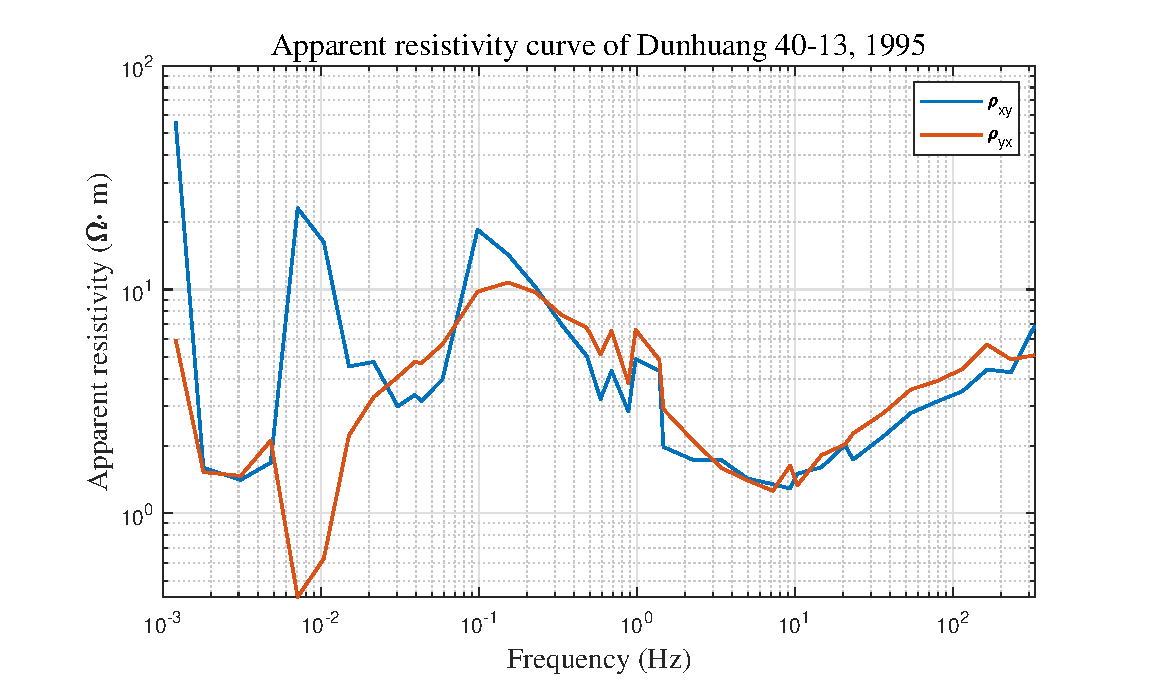
\includegraphics[width=0.95\columnwidth]{figures/r40-13.eps}
    \caption{The frequency-apparent resistivity curve  using the Dunhuang 1995 40-13 data.}
    \label{fig:r40-13}
\end{figure}

It can be seen from the figure that the apparent resistivity 1 and 2 are not equal, which may be caused by the anisotropy of the underground medium. The apparent resistivity reflects limited information, so it is also necessary to supplement it with a phase curve, as shown in Figure.\ref{fig:ph40-13}

\begin{figure}[htbp]
    \centering
    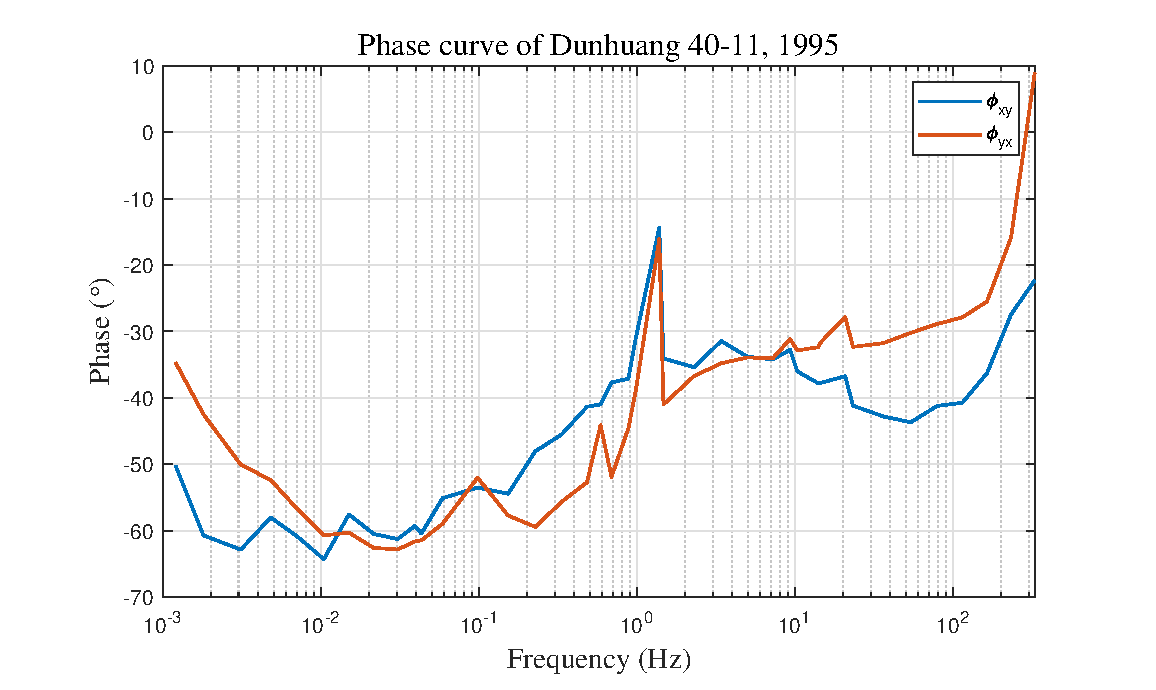
\includegraphics[width=0.95\columnwidth]{figures/ph40-13.eps}
    \caption{The frequency-phase curve using the Dunhuang 1995 40-13 data.}
    \label{fig:ph40-13}
\end{figure}

The calculation formula of the coherence of the full information vector is given by Equation.\eqref{cp}, and the impedance can be calculated in four ways, which can analyze the size of the noise in the data and the quality of the measured data. The image plotted by the measured data is shown in Figure.\ref{fig:cp40-13}.

\begin{equation}
    \label{cp}
    \mathrm{CP}_{uv} = 1-\dfrac{\sum^4_{k=1}|\overline{Z_{uv}}-Z_{uv}^k|}{4\overline{|Z_{uv}|}}
\end{equation}

\begin{figure}[htbp]
    \centering
    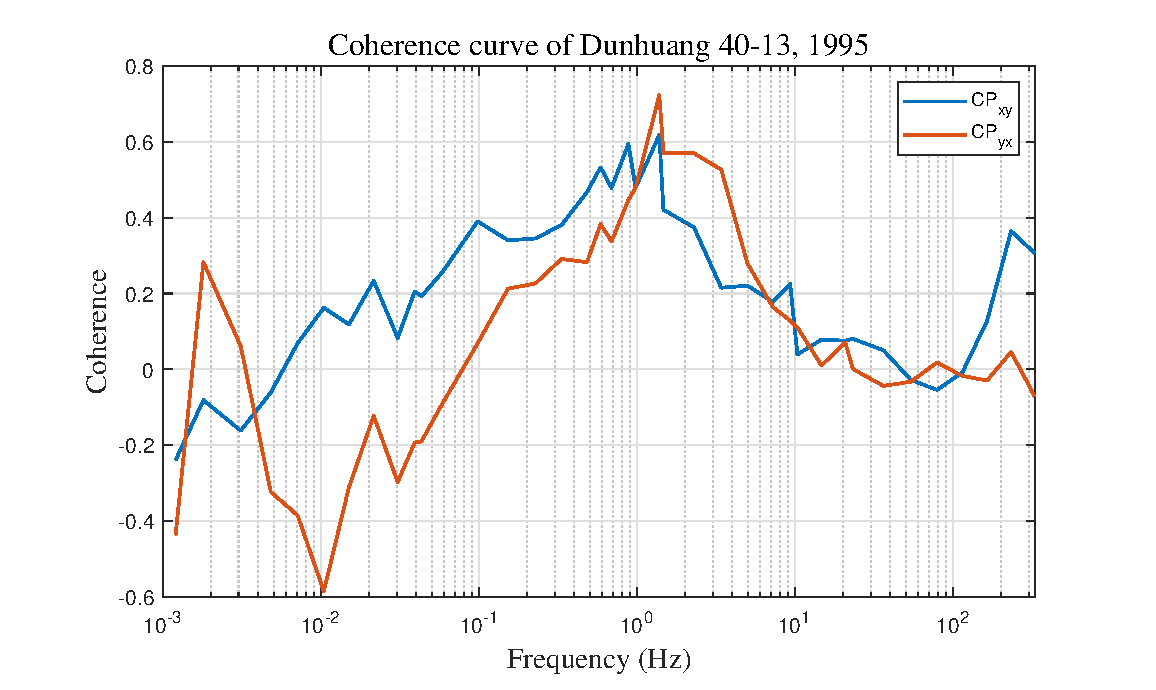
\includegraphics[width=0.95\columnwidth]{figures/cp40-13.eps}
    \caption{The coherence curve using the Dunhuang 1995 40-13 data.}
    \label{fig:cp40-13}
\end{figure}

It can be seen that the quality of the measured data is not good, and the deviation between the coherence degree and 1 is large. And we calculated the amplitude and phase of the tipper, as shown in Figure.\ref{fig:tp40-13}.

\begin{figure}[htbp]
    \centering
    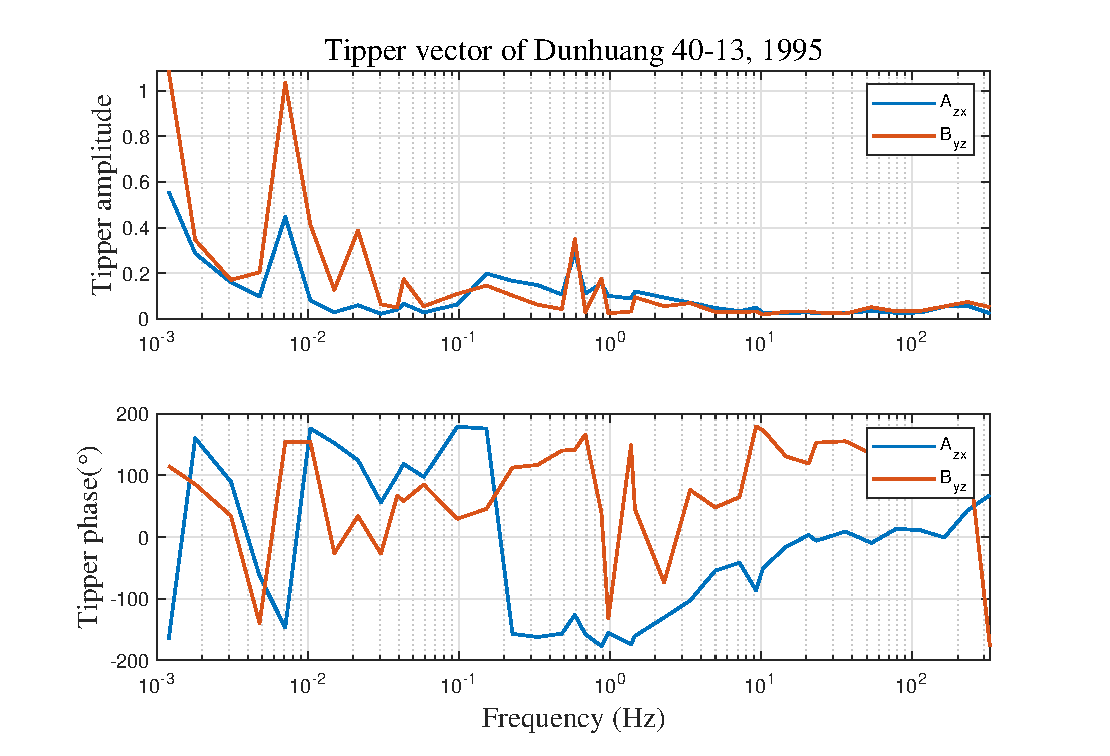
\includegraphics[width=0.95\columnwidth]{figures/tp40-13.eps}
    \caption{The amplitude and phase of the tipper using the Dunhuang 1995 40-13 data.}
    \label{fig:tp40-13}
\end{figure}

We calculated 13 measuring points of line 40 and plotted the frequency-apparent resistivity curve, as shown in Figure.\ref{fig:Line40}.

\begin{figure*}[htpb]
    \centering
    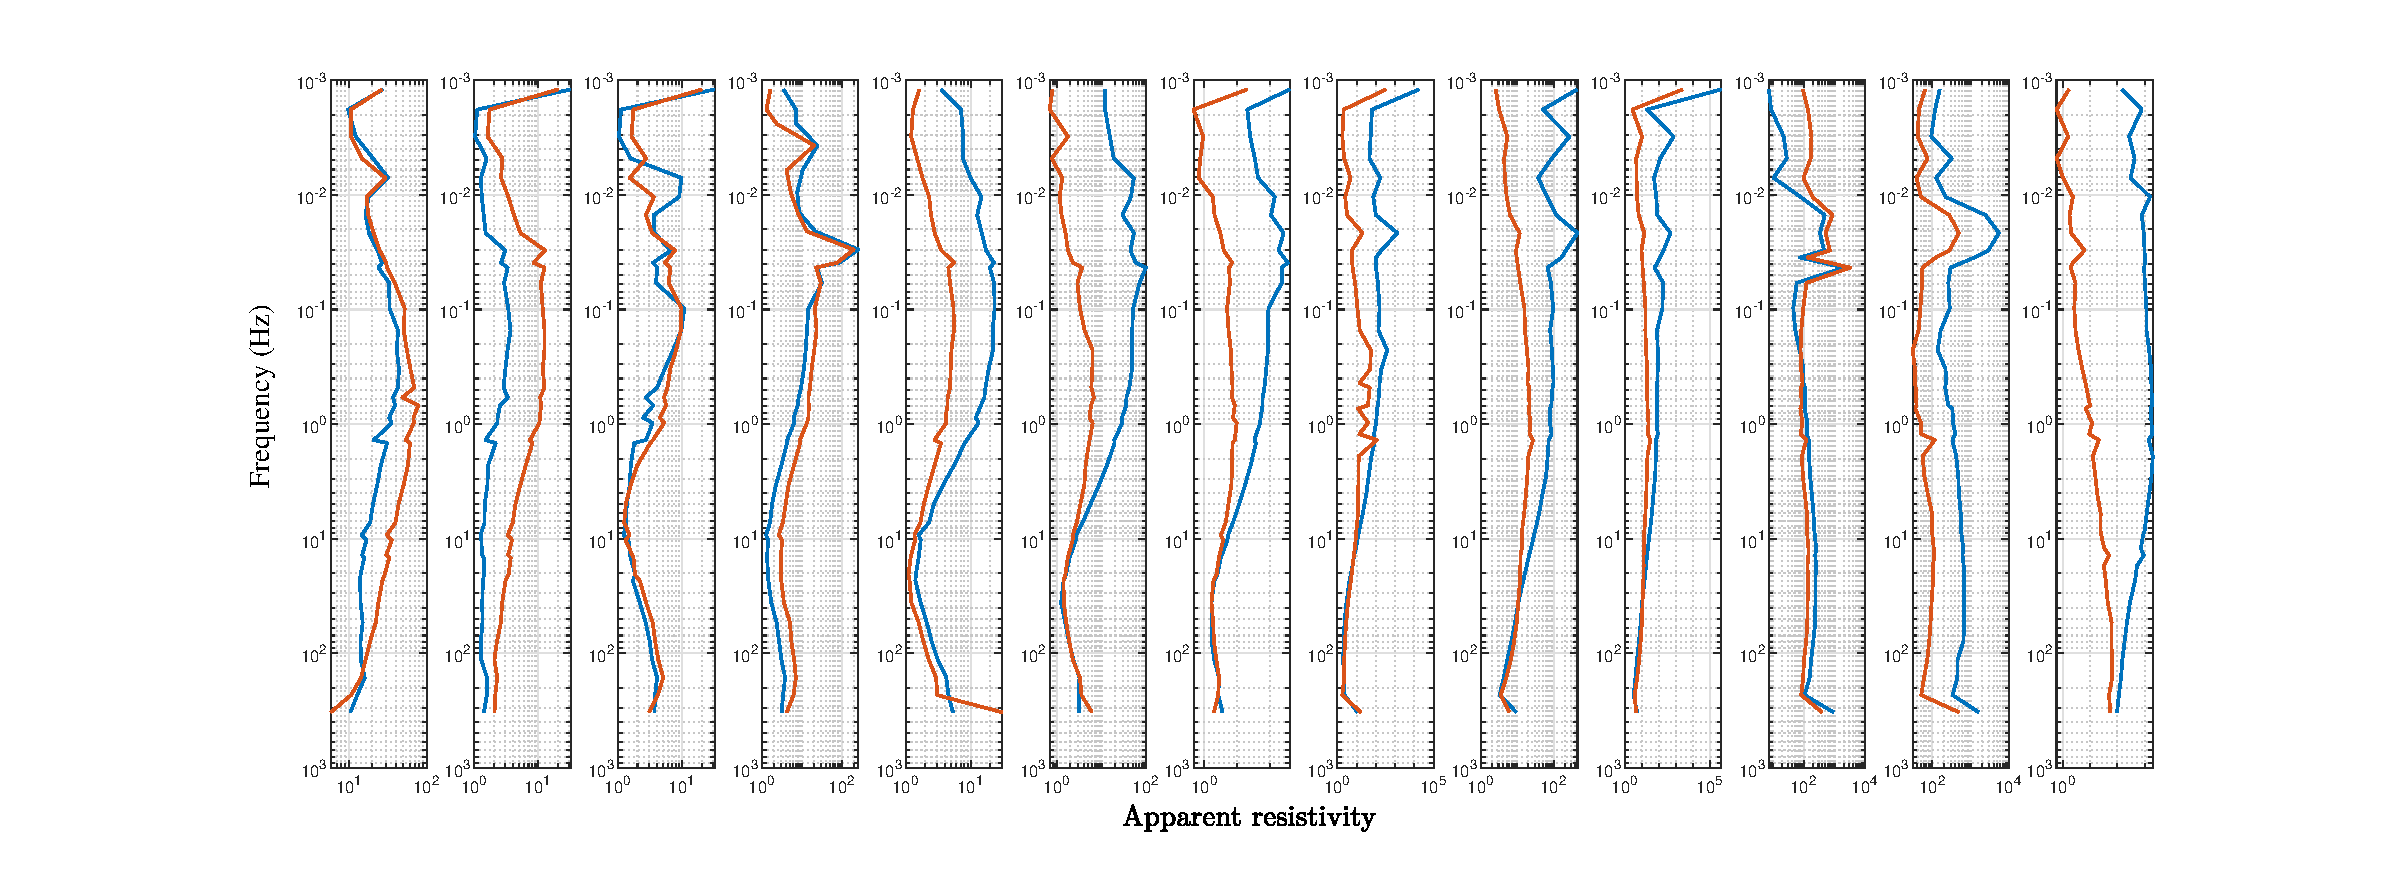
\includegraphics[width=0.95\textwidth]{figures/Line40.eps}
    \caption{The frequency-apparent resistivity curve of line 40.}
    \label{fig:Line40}
\end{figure*}

Then we use Bostick inversion algorithm for one-dimensional apparent resistivity sounding. This method is characterized by simple calculation but poor accuracy, which can be used as a basis for further calculation in the later period. Its formula is given by Equation.\eqref{Bostick1}.

\begin{equation}
    \label{Bostick1}
    h = \sqrt{\dfrac{\rho_\alpha}{2\pi f \mu}}
\end{equation}
\begin{equation}
    \label{Bostick2}
    \rho = \rho_\alpha\left(\dfrac{90^\circ}{\phi_\alpha}-1\right)
\end{equation}

The calculation results are shown in Figure.\ref{fig:bostick1} and Figure.\ref{fig:bostick2}.

\begin{figure}[H]
    \centering
    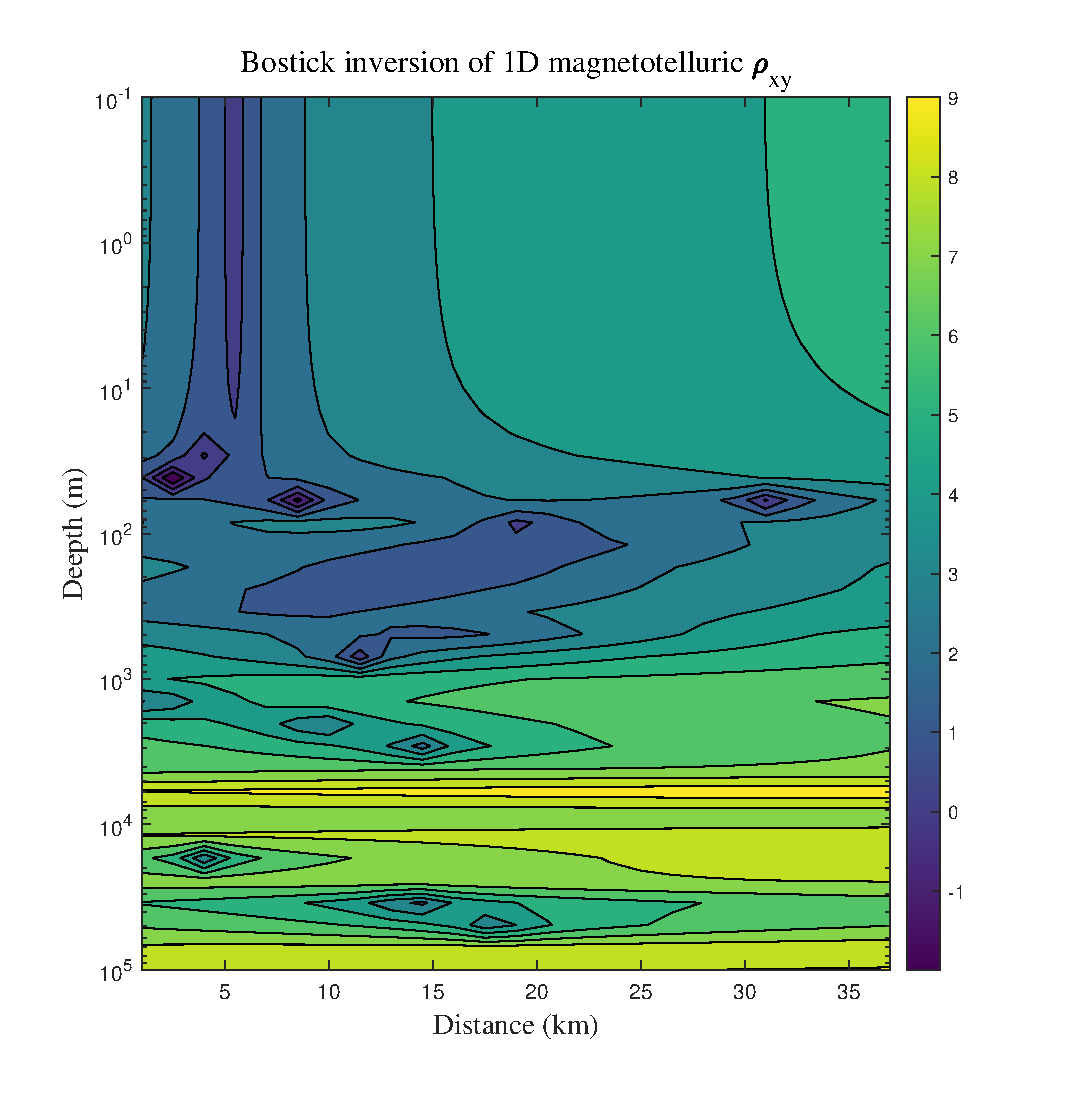
\includegraphics[width=0.95\columnwidth]{figures/Bostick1drxy.eps}
    \caption{The resistivity $\rho_{xy}$ curve of line 40 using 1d-Bostick inversion algorithm.}
    \label{fig:bostick1}
\end{figure}

\begin{figure}[H]
    \centering
    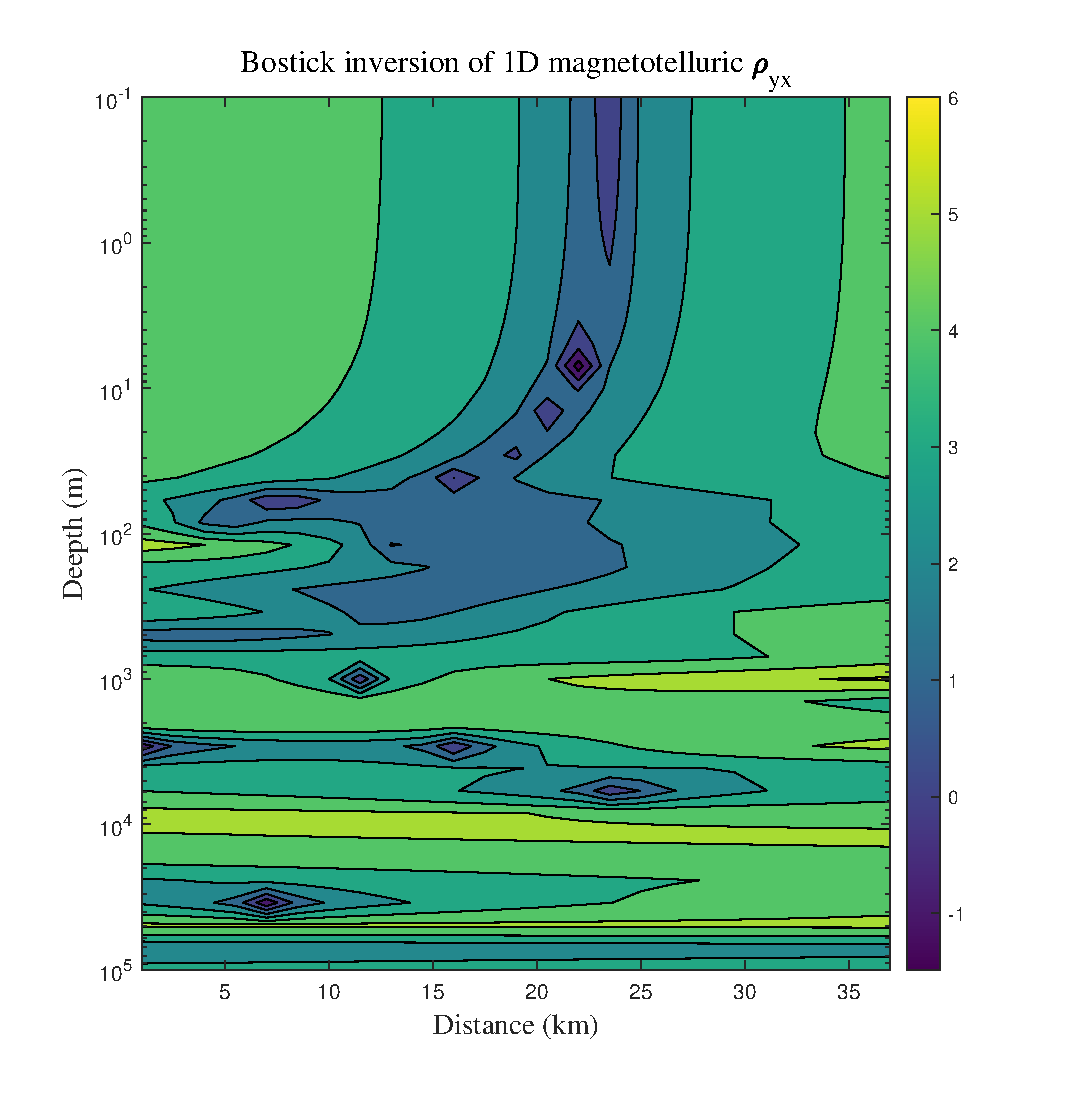
\includegraphics[width=0.95\columnwidth]{figures/Bostick1dryx.eps}
    \caption{The resistivity $\rho_{yx}$ curve of line 40 using 1d-Bostick inversion algorithm.}
    \label{fig:bostick2}
\end{figure}

The above calculation results are based on the available power spectrum data. At the same time, magnetotelluric sounding based on the time series of electric and magnetic field intensity is also calculated, and the 1-d bostick apparent resistivity inversion is performed.

\begin{figure}[htbp]
    \centering
    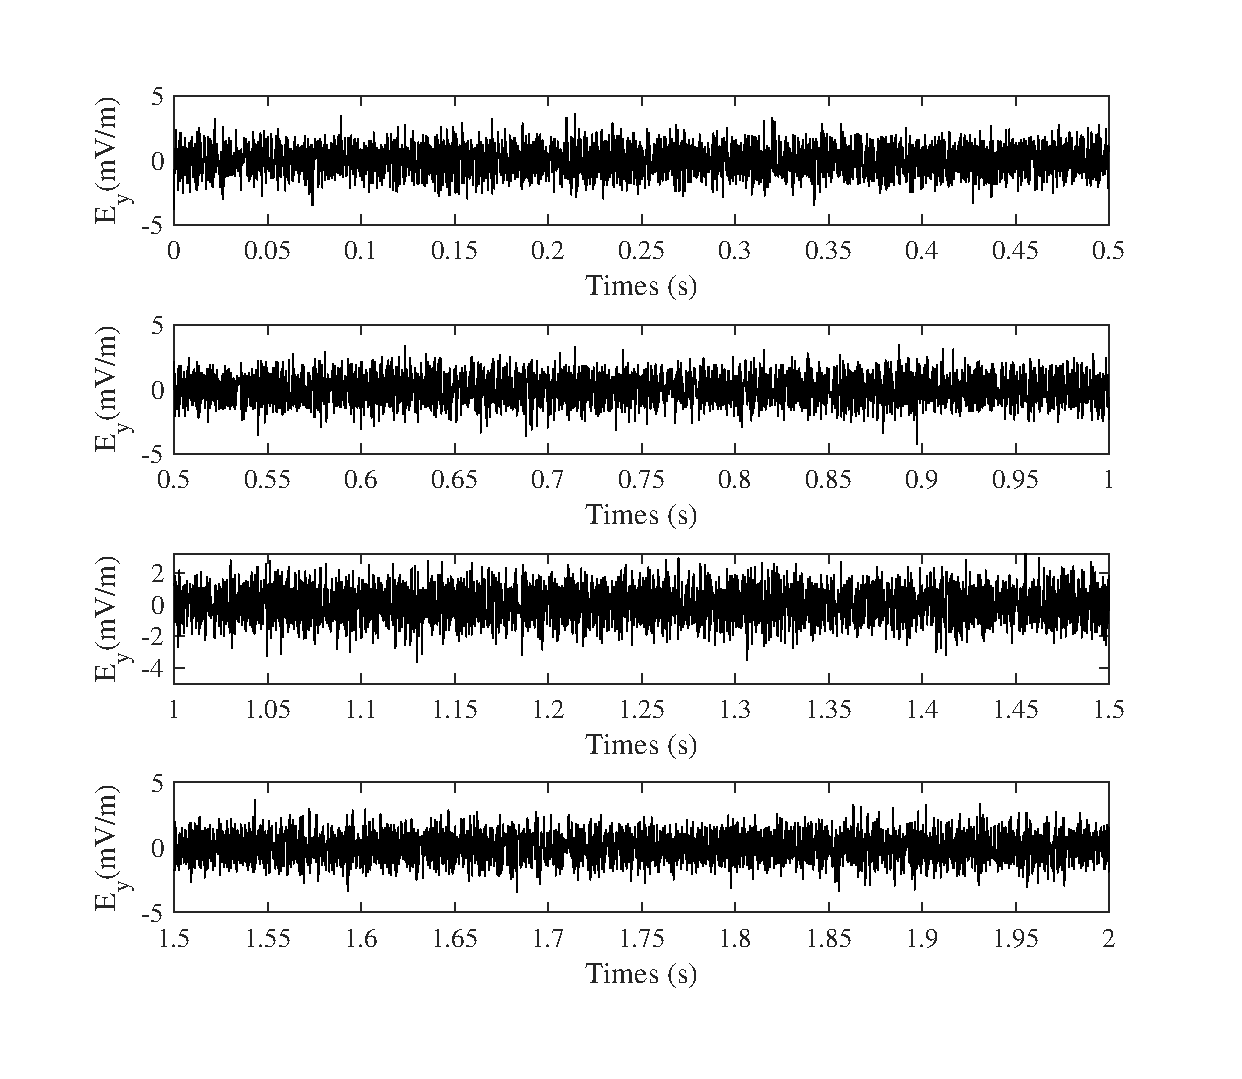
\includegraphics[width=0.95\columnwidth]{figures/et.eps}
    \caption{Electric field strength time series of 0 to 1 second, sampling frequency 4096Hz.}
    \label{fig:et}
\end{figure}

As a supplement to our assignment, we also used additional data \texttt{YJBey.dat} and \texttt{YJBhx.dat}. This set of data gives the electric field strength and magnetic field strength of the time series. The sampling frequency of each channel is 4096Hz and the sampling time is 2 seconds. In order to use linear least squares estimation calculation, we take 0.5s as the time interval to obtain 4 sets of electric field strength and magnetic field strength data. By fast Fourier transform of the time series, four power spectra are obtained, as shown in the Figure.\ref{fig:ef}.

\begin{figure}[htbp]
    \centering
    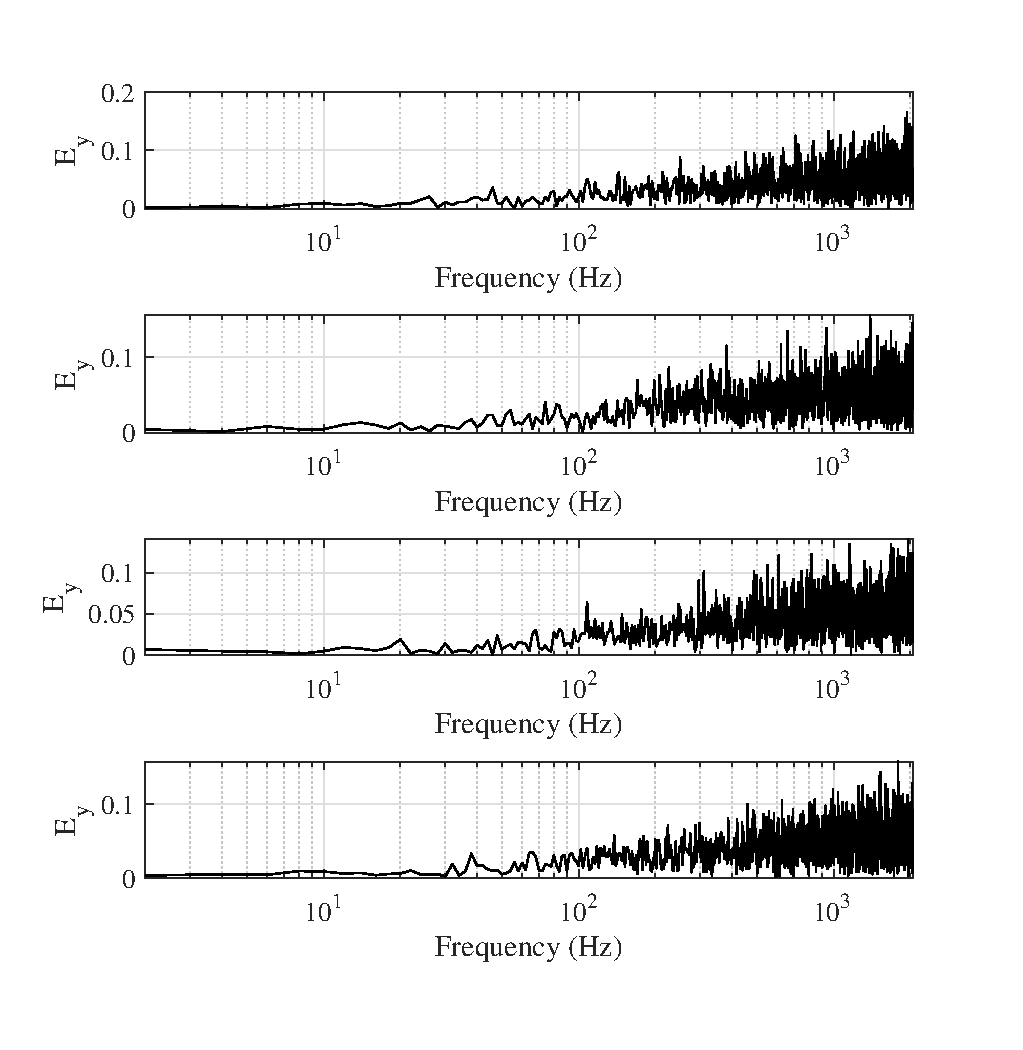
\includegraphics[width=0.95\columnwidth]{figures/ef.eps}
    \caption{Amplitude spectrum of electric field intensity}
    \label{fig:ef}
\end{figure}

The calculated apparent resistivity curve and phase curve are shown in the Figure.\ref{fig:yjb-ra} and Figure.\ref{fig:yjb-ph}.

\begin{figure}[htbp]
    \centering
    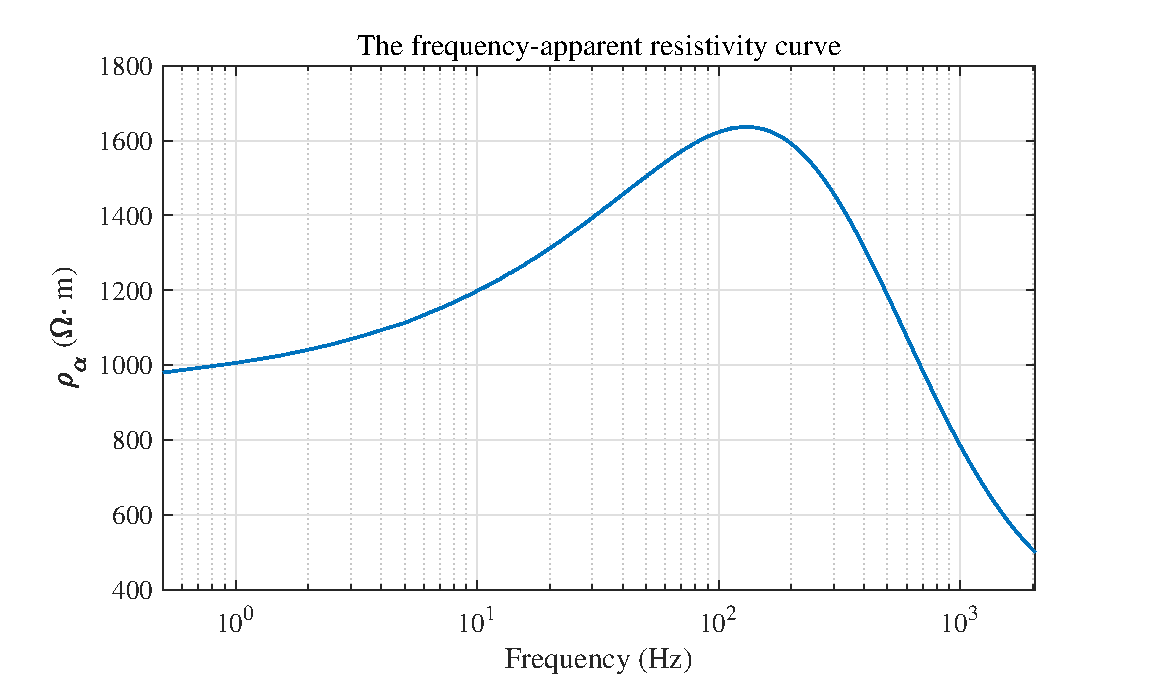
\includegraphics[width=0.95\columnwidth]{figures/YJBra.eps}
    \caption{The apparent resistivity curve.}
    \label{fig:yjb-ra}
\end{figure}

\begin{figure}[htbp]
    \centering
    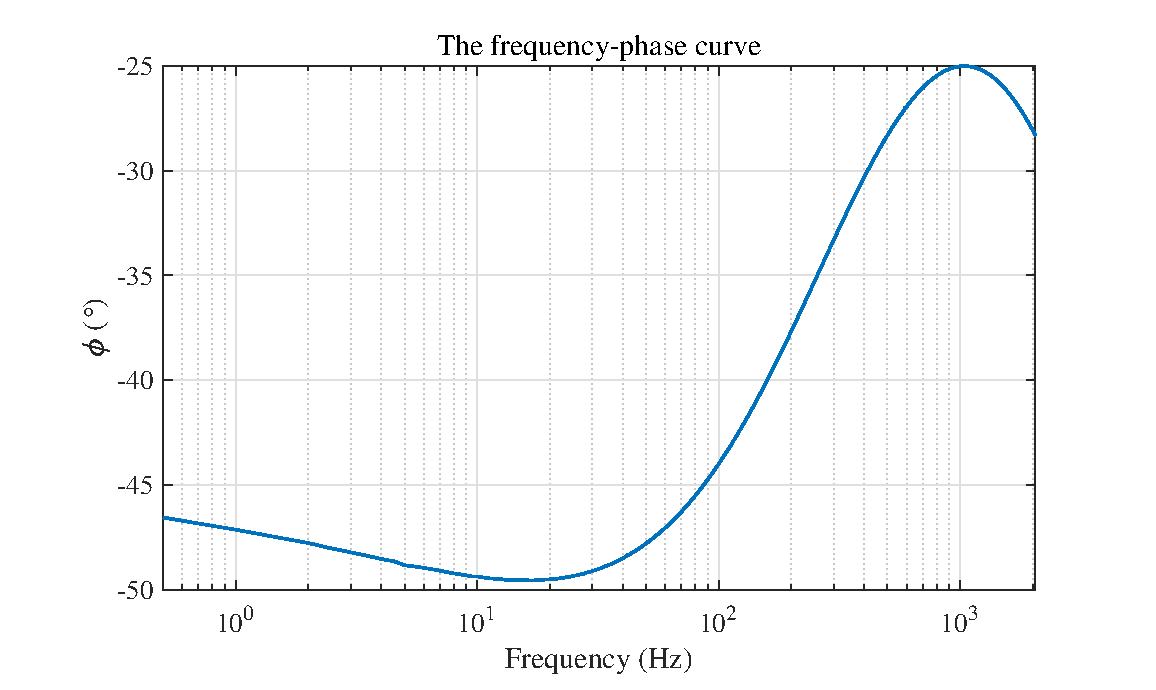
\includegraphics[width=0.95\columnwidth]{figures/YJBph.eps}
    \caption{The phase curve.}
    \label{fig:yjb-ph}
\end{figure}

Again, a one-dimensional bostick inversion is performed on this result to obtain the underground resistivity, as shown in the Figure.\ref{fig:yjb-r}.

\begin{figure}[htbp]
    \centering
    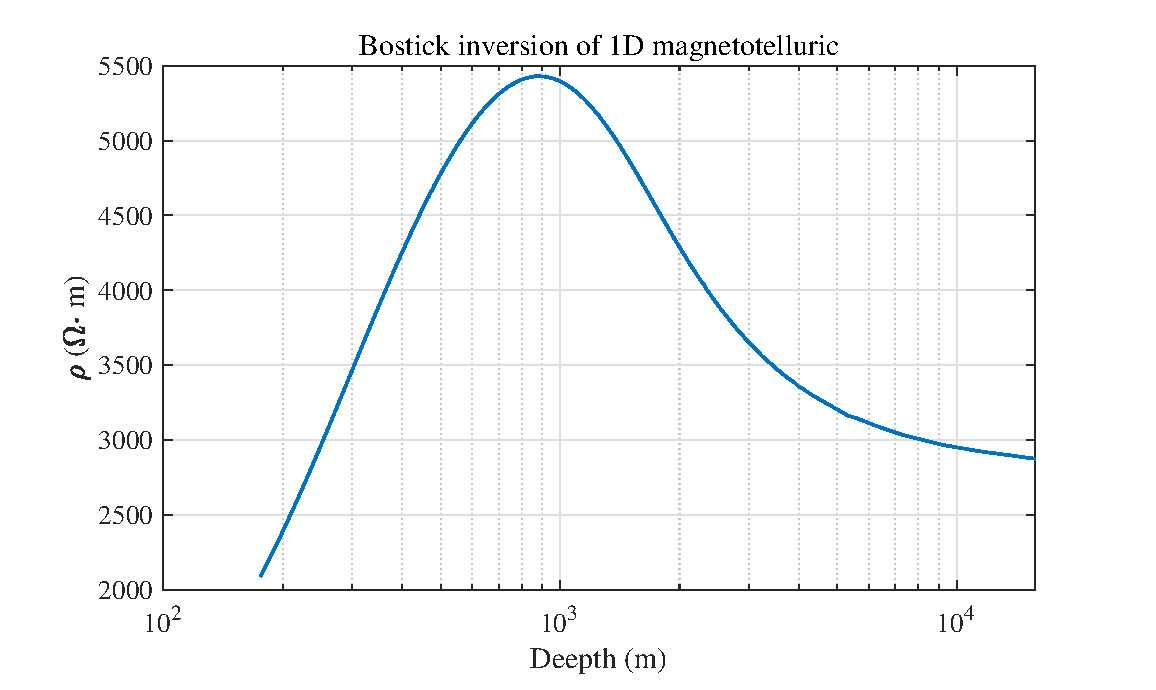
\includegraphics[width=0.95\columnwidth]{figures/YJBbostick.eps}
    \caption{One-dimensional bostick inversion result curve.}
    \label{fig:yjb-r}
\end{figure}

\section{Conclusions}

In this semester's assignment, we derived the linear least squares estimation formula for impedance in the magnetotelluric method. Using this formula, we calculated the apparent resistivity curve and phase curve for the 1995 Dunhuang Line 40 data, as well as the coherence and tipper vector. Based on the coherence analysis, it was found that the data quality was suboptimal, leading to significant deviations in the results obtained from one-dimensional Bostick inversion. Additionally, we processed magnetotelluric sounding data from supplementary operations, performing one-dimensional Bostick inversion which yielded satisfactory results.

Through this semester's project, team members gained a deeper understanding of the fundamental theory and practical applications of the magnetotelluric method. We also acquired skills in impedance estimation and necessary programming techniques. Furthermore, our comprehension of forward and inverse modeling in electrical exploration has been significantly enhanced.

\section{Acknowledgements}

Professor Jiabin Yan gave guidance for this assignment. Researcher Xiaozhong Tong provided rich and valuable suggestions for group. Professors Haifei Liu and Rujun Chen also provided advice to the group.

\begin{rhoenv}[frametitle=Code availability]
    The source codes are available for downloading at the link: https://github.com/PourRevenir/Magnetotelluric-Signal-Processing, required software MATLAB R2024a.
\end{rhoenv}

    % \begin{rhoenv}[frametitle=Environment with custom title]
    %     Hello! I am an example of the \textit{rhoenv} included in rhoenvs \LaTeX\ package. Here you can include relevant information or notes about your work. You can modify my title directly in the code.
    % \end{rhoenv}
    
        
    % \begin{figure}[htbp]
    %     \centering
    %     \includegraphics[width=0.71\columnwidth]{Example.pdf}
    %     \caption{Example figure obtained from PGFPlots \cite{PFGPlots}.}
    %     \label{fig:figure}
    % \end{figure}

    % \begin{table*}[pb]
    %     \RaggedRight
    %     \caption{Table example that covers the width of the page.}
    %     \label{tab:table}
    %         \begin{tabular}{lllp{12.2cm}}
    %             \toprule
    %             \textbf{Day} & \textbf{Min Temp} & \textbf{Max Temp} & \textbf{Summary} \\ 
    %             \midrule
    %             Monday & 11\textdegree C & 22\textdegree C & A clear day with lots of sunshine.  Strong breeze will bring down the temperatures. \\
    %             Tuesday & 9\textdegree C & 19\textdegree C & Cloudy with rain, across many northern regions. \\
    %             Wednesday & 10\textdegree C & 21\textdegree C & Rain will still linger for the morning. 
    %             Conditions will improve by early afternoon and continue 
    %             throughout the evening.\\
    %             \bottomrule
    %         \end{tabular}
            
    %     \tabletext{Note: Obtained from \LaTeX\ tables \cite{projects-2023}.}
        
    % \end{table*}

    % \nolinenumbers
    % \lstinputlisting[caption=Example of matlab code., label={lst:listing-Mat}, language=Matlab]{example.m}
    % \linenumbers
    
    % \nolinenumbers
    % \begin{lstlisting}[language=TeX, caption=Alternative unnumbered section.]
    % \titleformat{name=\section,numberless}[block]
    %     {\color{rhocolor}\sffamily\large\bfseries}
    %     {}
    %     {0em}
    %     {#1}
    %     []
    % \end{lstlisting}
    % \linenumbers

%----------------------------------------------------------

\printbibliography

%----------------------------------------------------------

\end{document}